%!TEX root = ../thesis.tex
%*******************************************************************************
%****************************** Second Chapter *********************************
%*******************************************************************************

\chapter{The SNO+ Detector}\label{chap:detector}
\epigraph{\textit{The light-soaked days are coming.}}{\textsc{John Green}}
\section{Detector Geometry and Design}
The SNO+ detector is a large, multi-purpose neutrino detector built in the SNOLAB underground laboratory near Sudbury, Canada. Its main detector structure is taken from the Nobel prize-winning Sudbury Neutrino Observatory (SNO)~\cite{}, % cite nobel prize for Art
which can be seen in Fig.~\ref{fig:snoplus_detector}. The bulk of the detector is the main detector medium, which changes depending on the phase of the experiment --- more on the specifics of this shortly. This medium is held within a \SI{12}{\metre} diameter sphere known as the Acrylic Vessel (AV). The AV floats within a body of ultra-pure water (UPW), beyond which is a stainless steel support structure (PSUP) that holds $\sim\num{9000}$ Photomultiplier Tubes (PMTs). It is these PMTs that detect the light generated from physics events that occur within the detector medium. The AV is kept in place relative to the PSUP through a series of `hold-up' and `hold-down' tensylon ropes. All of these components are suspended within a large cylindrical cavity also filled with UPW. Directly above the detector is the Deck, within which all the detector electronics are kept. Access within the AV for calibration tools and filling is possible only through the acrylic `neck' on top of the AV.

\begin{figure}
    \centering
    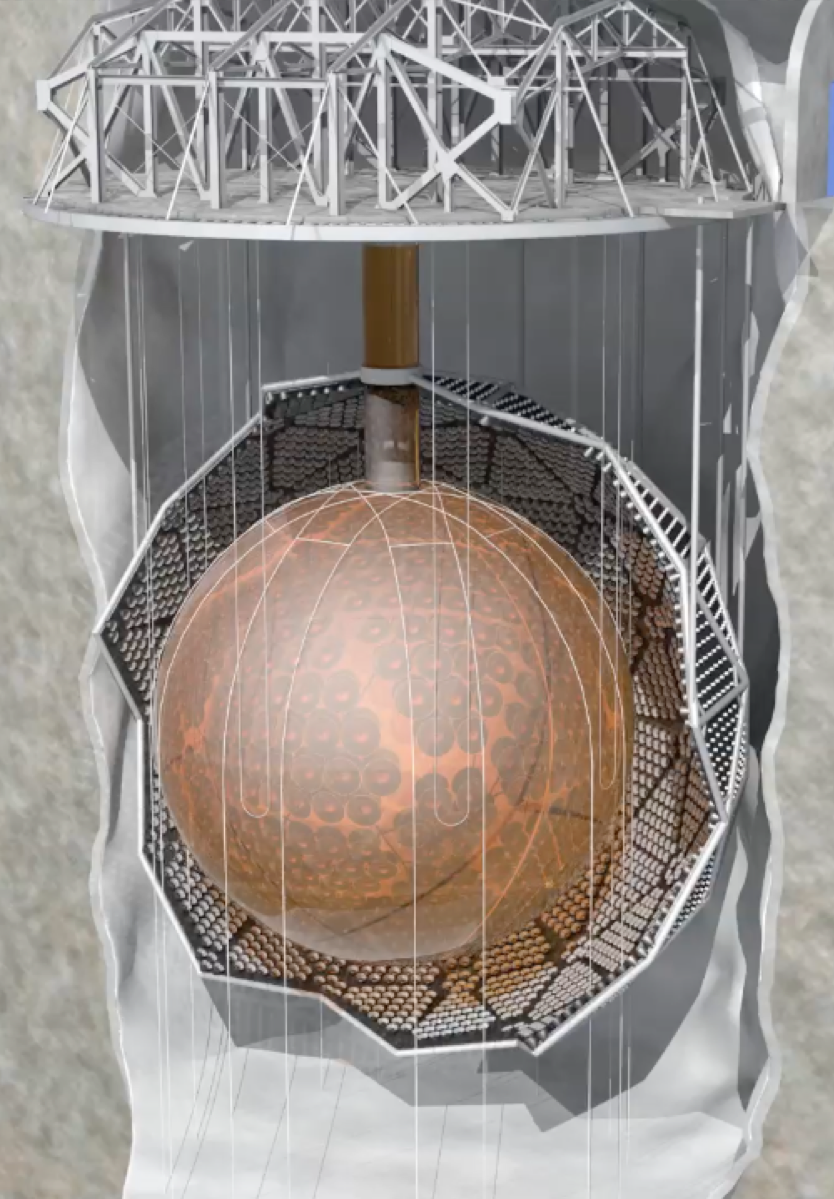
\includegraphics[width=0.48\linewidth]{2_Detector/Figs/detector_picture.png}
    \caption[3D model of the SNO+ detector]{3D model of the SNO+ detector~\cite{albanese_sno_2021}.}
    \label{fig:snoplus_detector}
\end{figure}

This choice of design is highly deliberate, with the details are discussed in~\cite{albanese_sno_2021}. 
The location \SI{2.2}{\km} underground ensures that there is minimal impact from cosmic rays: only 3 cosmic ray muon events are expected within the detector an hour~\cite{}. % cite something - Lorna's thesis?
By making the detector spherical, the high degree of symmetry can easily be taken advantage of in event reconstruction and analysis. Moreover, light produced throughout most of the body of the AV will be minimally-impacted by refraction through the acrylic. The only major exception to this is light emitted within $\sim\SI{50}{\cm}$ of the AV, at which point total internal reflection becomes possible. In order to make as much emitted light be able to get detected as possible, all materials within the PSUP were chosen for their optical transparency (excepting the ropes).

Another major design consideration is that of radioactive backgrounds. Maintaining minimal levels of backgrounds is critical for effective particle physics, otherwise the signal one is searching for would become completely swamped. Materials within the detector were chosen to ensure these background levels would be low enough for the Collaboration's physics goals to be achieved. Another benefit of the spherical design is its high volume-to-surface area ratio, which means that the relatively-high background levels of the PMT glass are kept far away from the detection medium.

\section{Experimental Phases}
As mentioned earlier, SNO+ was designed to fulfil a number of physics goals over multiple `phases' of the detector's lifetime. The phases are distinguished by the medium that fills the AV. The first main phase (after a brief `air-filled' phase used only for detector commissioning) was that of the `water-fill', with data taken between May 2017 and July 2019. This was used to perform fundamental optical calibrations of the detector~\cite{}, % Water optics paper
measurements of the solar neutrino flux~\cite{}, % water solar papers
observation of neutrino oscillations in reactor anti-neutrinos~\cite{}, % water antinu paper
and searches for nucleon decay~\cite{}. %nucleon decay papers

After this, the detector was filled with 800 tonnes of liquid scintillator known as linear alkylbenzene (LAB), mixed with the fluor PPO. More information on the physics of scintillators can be found in Section~\ref{sec:interactions_w_matter}. Filling of the LABPPO cocktail had to be paused in March 2020 due to the COVID-19 pandemic, leading to the detector having its bottom half still filled with UPW, and the top half filled with LAB and PPO at \SI{0.5}{\gpl}. This impromptu phase became known as the `partial-fill', and allowed for some creative analyses to be performed: an initial neutrino oscillation analysis from reactor anti-neutrinos~\cite{}, % Iwan's thesis & forthcoming paper
as well as the first ever observation of directionality in a high light yield scintillator~\cite{}. % Josie's thesis & forthcoming PRL
Eventually, filling of the detector with liquid scintillator was able to resume, being completed in May 2021. At that point, the concentration of PPO in the detector was at \SI{0.6}{\gpl}, markedly below the target level of \SI{2.0}{\gpl}. A further `PPO top-up' campaign then proceeded, finishing in April 2022 with a final concentration of \SI{2.2}{\gpl} PPO. Thus began the `scintillator-fill' of the experiment, which continues on during the time of writing. The main goals for this phase include a number of solar neutrino analyses (including the one described in Chapter~\ref{chap:solar_osc_analysis}), a precision measurement of the neutrino oscillation parameter \dmsq{} using reactor anti-neutrinos~\cite{}, % Iwan's thesis
and further calibrations of the detector and its backgrounds.

Finally, in the near future the detector will be loaded with Tellurium, allowing for the flagship analysis of the experiment to begin: neutrinoless double-beta decay. The details of this chemical loading process are described in~\cite{}. % Te loading paper
Alongside the Te-loaded liquid scintillator will be a number of other chemicals within the scintillator cocktail that will help ensure optimal optical properties and chemical stability. These include: the surfactant DDA to ensure the solubility and stability of the `Te-diol' within the LAB; the wavelength-shifter BisMSB to absorb light at short wavelengths and re-emit closer to the optimal quantum efficiency of the detector's PMTs; and the anti-oxidant BHT to prevent any free-radicals within the liquid scintillator from `yellowing' the medium.

% \begin{itemize}
%     \item Describe the SNO+ geometry at a high level: explain structure, and why certain design choices were made.
%     \item Describe standard coordinate axis; note AV offset.
%     \item Mention the main phases of SNO+, both past, present, and future.
% \end{itemize}
\section{Detecting a Physics Event in SNO+: A Journey}
To understand well the SNO+ detector, it is worth thinking about how the information of a physics event, e.g. a solar neutrino interaction, gets observed. This section follows the journey of such an event.
\subsection{Particle Interactions with Matter}\label{sec:interactions_w_matter}
All observable physics events within the detector begin by the generation of some form of ionising radiation: $\alpha$, $\beta^{\pm}$, $\gamma$, $p$ or $n$. These can be created via numerous processes, both exciting (e.g. \onbb{} or interactions of neutrinos) and banal (e.g. decay of background radioisotopes): see Section~\ref{sec:background_processes} for some of them. Regardless of their origin, these particles begin propagating through the detector, and interacting with the detector medium. A number of mechanisms then allow for the generation of optical-wavelength light as a result of these interactions.
\subsubsection{Cherenkov Light Emission}
Whenever a charged particle passes through a dielectric medium, nearby molecules polarise and attempt to align their dipoles in the direction of the charge. This results in a temporary polarisation of the medium as the charge passes though it. However, the molecules can only respond to the charge's movement at the speed of light in the medium, which is necessarily slower than the speed of light in a vacuum by a factor of the medium's refractive index. If the charged particle is able to move at a speed greater than the speed of light in the medium, then the dipoles formed within the medium struggle to respond to the motion. This superluminal motion results in a wake of polarisation in the medium, which propagates outwards from the direction of the charged particle: this is Cherenkov light. This process is much akin to the `sonic boom' that occurs when an object travels at supersonic speeds.

Cherenkov light emanates outwards in a cone along the direction of the charge's travel; the angle of the cone $\theta_{\gamma}$ is purely a function of the speed of the charged particle relative to the speed of light, $\beta$, and the refractive index of the medium $n(\lambda)$: $\cos{\theta_{\gamma}}(\lambda) = \frac{1}{n(\lambda)\beta}$. This formula also demonstrates that there is a minimum speed necessary for Cherenkov light to be generated: $\beta = 1/n(\lambda)$.

All detection media are capable of allowing for Cherenkov light to be generated, as long as sufficiently high energy particles can be produced. In the water-fill phase of the detector, Cherenkov light was the only means by which light could be generated. Light from Cherenkov emission can still be created in liquid scintillator, but it tends to be swamped by another form of light generation: scintillation.
\subsubsection{Scintillation}
Whenever a high-energy particle passes through a medium, interactions between the particle and the medium's molecules lead to an inexorable transfer of energy from the former to the latter. These interactions are numerous, and are a function of the type of particle and its kinetic energy. For example, a \SI{5}{\MeV} electron loses energy from electromagnetic interactions with nearby molecules as it passes through, and scatters after colliding with atomic electrons or nuclei. From the perspective of the medium, its molecules use this new-found energy for a number of activities:
\begin{enumerate}
    \item Exciting atomic electrons into various higher-energy states;
    \item Ionising atomic electrons;
    \item Increasing the overall kinetic energy of the molecule.\label{enum:heat}
\end{enumerate}
At the macroscopic level, process~\ref{enum:heat} is simply the conversion of the high energy particle's energy into heating the medium. In fact, within most materials the other processes also end up doing the same.

However, for certain special classes of material the excitation and ionisation of electrons can lead to a unique process: scintillation (often generally referred to as `luminescence' or `fluorescence'). Here we choose to focus on the particular case of organic liquid scintillators, given that this is the type of scintillator which currently fills the SNO+ detector. Certain organic compounds (i.e. molecules built from a skeleton of carbon atoms) have `$\pi$-bonds' in addition to the single `$\sigma$-bond' that is needed to bond two carbon atoms together. A major example of these $\pi$-bonds is in the benzene rings of `aromatic' hydrocarbons, such as LAB and PPO. Fig.~\ref{fig:benzene_pi_bonds} shows an image of the orbitals for these $\pi$-bonds in a benzene ring: note how the electrons that inhabit these particular orbitals become entirely delocalised.

\begin{figure}
    \centering
    % \includegraphics[]{}
    \caption[]{}
    \label{fig:benzene_pi_bonds}
\end{figure}

Because of this delocalised structure, excited atomic $\pi$-electrons can stay in what is typically the first-excited state for somewhat longer than typical excited states: lifetimes of $\mathcal{O}(\SI{e-9}{\second})$ as opposed to $\mathcal{O}(\SI{e-12}{\second})$. Moreover, decays from this state can emit light typically in the optical-wavelength range. It is this light emission that is called `scintillation light'. Ionised electrons can also 

{
    \color{blue}
    \begin{itemize}
        \item Begin the ``journey of a SNO+ Physics Event'' --- starting by explaining how a high-energy particle interacts with matter to generate Cherenkov and/or scintillation light. In both cases, optical wavelength light gets generated.
        \item Then, light propagates through the detector, possibly undergoing various physics processes: Rayleigh scattering, absorption, re-emission, refraction, and reflection.
        \item Light gets detected via the PMTs: explain how.
        \item Thus begins the DAQ chain. Signals reach the crates of electronics on deck and are processed. A ``sufficient signal'' leads to the triggering of the detector, which then enables for the saving of the event's information via the event builder.
    \end{itemize}
    \section{Calibrations and Detector Modelling}
    \begin{itemize}
        \item I will now describe how calibrations enable us to use the stored data for actual physics.
        \item Detector's state is continuously monitored via a number of systems for data quality purposes, including a human detector `shifter'. Mention use of run numbers. CHS and CSS ensure only ``good'' channels used in any analysis.
        \item First main set of calibrations are the ECAs and PCAs. These help us convert raw electronic signal information from PMTs into `calibrated' hit times and charges. PCAs performed via TELLIE and the Laserball.
        \item These initial calibrations allow for the first two passes of data processing. SMELLIE data comes from this part of the processing chain.
        \item In order to infer properties of an underlying physics event, an accurate model of the detector is needed. This requires two things: a set of calibration tools, and a piece of simulation software. The latter is RAT (explain briefly).
        \item Aims of remaining calibration tools are to obtain the optical parameters necessary for accurate modelling. Go through briefly all the calibration tools we have available: SMELLIE, AMELLIE, the Laserball, the AmBe and N16 sources, and in situ backgrounds.
        \item Using RAT once calibrated, event reconstruction can become possible. Briefly describe how energy, position, and time reconstruction works. Mention existence of direction fitting!
    \end{itemize}
}
